%!TEX root = ../main.tex

In this section the way in which the effectiveness of the method will be measured is explained, the measure of success and the scope of the method will be described. In terms of scope the aim of the method is to produce plausible lighting for Augmented Reality applications, and thus increase the sense of realism of the composed graphics. This does not mean that imagery that would for all practical purposes be indistinguishable from reality will be achieved. As said earlier, the incompatible lighting is only one of the problems with current AR graphics. In order to achieve complete realism all the other problems would have to be tackled as well, this includes occlusion from real objects as the most prominent one, but also the shadows of real objects not affecting the virtual ones at all. The method will also not attempt to improve other aspects of AR, such as tracking. The method comprises a pre-calculation and a real-time phase, pre-calculation being the acquisition of the 360 panorama and its analysis for calculation; real-time is the actual rendering. It is also desirable and expected that the pre-calculation phase can be completed within a reasonable time frame on a mobile device, in terms of usability this should be no more than 1 minute.\newline
\section{Setup}
In order to test the results a similar setup as the one shown in figures 2 and 3 will be used, showing real objects made out of different materials, so at least a matte, a shiny and a reflective object are present. The scene will be augmented with a virtual object with the possibility of changing the shader used for it. At least a Lambert diffuse, a Phong or Blinn and a specular shaders will be available. The setup will have known,  consistent and controllable lighting.\newline
Besides augmenting the scene with the developed application images will be produced manually, replicating the real world lighting as close as possible. Screen captures of the plain real world scene, with no augmentation whatsoever; the manually augmented scene and the automatic results provided by the method will be left for the reader to see. Also criticizing and discussing how much the results obtained match the expected results and the ground truth. Another additional image will be taken using the commercial solution Vuforia as engine for augmentation, in order to compare the method to already existing solutions.\newline
The actual way in which the experiment will be conducted is defined in the following scenario:
\begin{itemize}
    \item \textbf{Setting:} A room with consistent and invariable lighting will be used. A set of common objects will be laid on a table, the objects must include a matte, a shiny and a reflective object. At least one extra light source with known parameters.
    \item \textbf{Requirements:} A mobile device running the developed demo application, a marker for virtual objects. A real object and its corresponding virtual counterpart, modelled as close as possible. 
    \item \textbf{Goals:} Obtaining a set of images that will enable readers and experimenters alike to make a fair comparison of the method application, a commercial solution and a real object.
    \item \textbf{Actions:} Place the real object on top of the marker and take a picture with the same device running the demo application. Then remove the object and take screen captures of the augmented scene using a commercial solution and subsequently the method demo application.
     \item \textbf{Benchmark:} The image result yielded by each method, as well as the time for the pre-processing phase (where applicable) and the time per frame will be captured and used for comparison's sake and benchmarking.
\end{itemize}

\section{Expected Results}
Since the final product is a graphic on a screen, an image, it's somewhat difficult to define a measure of success, due to the inherent subjective nature of image appreciation. It can be said that the method successfully converged if in the final image the synthetic objects are hard to tell from the real ones, if formed on a line on a still image. Hard to tell meaning that some scrutiny and reflection is necessary when looking at a screen capture of the application. If an average technology consumer is able to immediately tell which of the objects are synthetic and which are real the method will then have failed. To explain the measure better in Figure 2 we can see three objects, 2 real, 1 synthetic, from an AR included with the Vuforia library. Figure 3 shows the same array of objects, again the same 2 real and 1 synthetic, but in this case the synthetic object having been inserted with hand tuned lighting. It can be appreciated that it is harder to differentiate the virtual object in the second image than on the first one.
\begin{figure}[H]
\centering
\includegraphics[width=0.6\textwidth]{Figures/fake.jpg}
\caption{Default lighting, making the virtual object stand out}
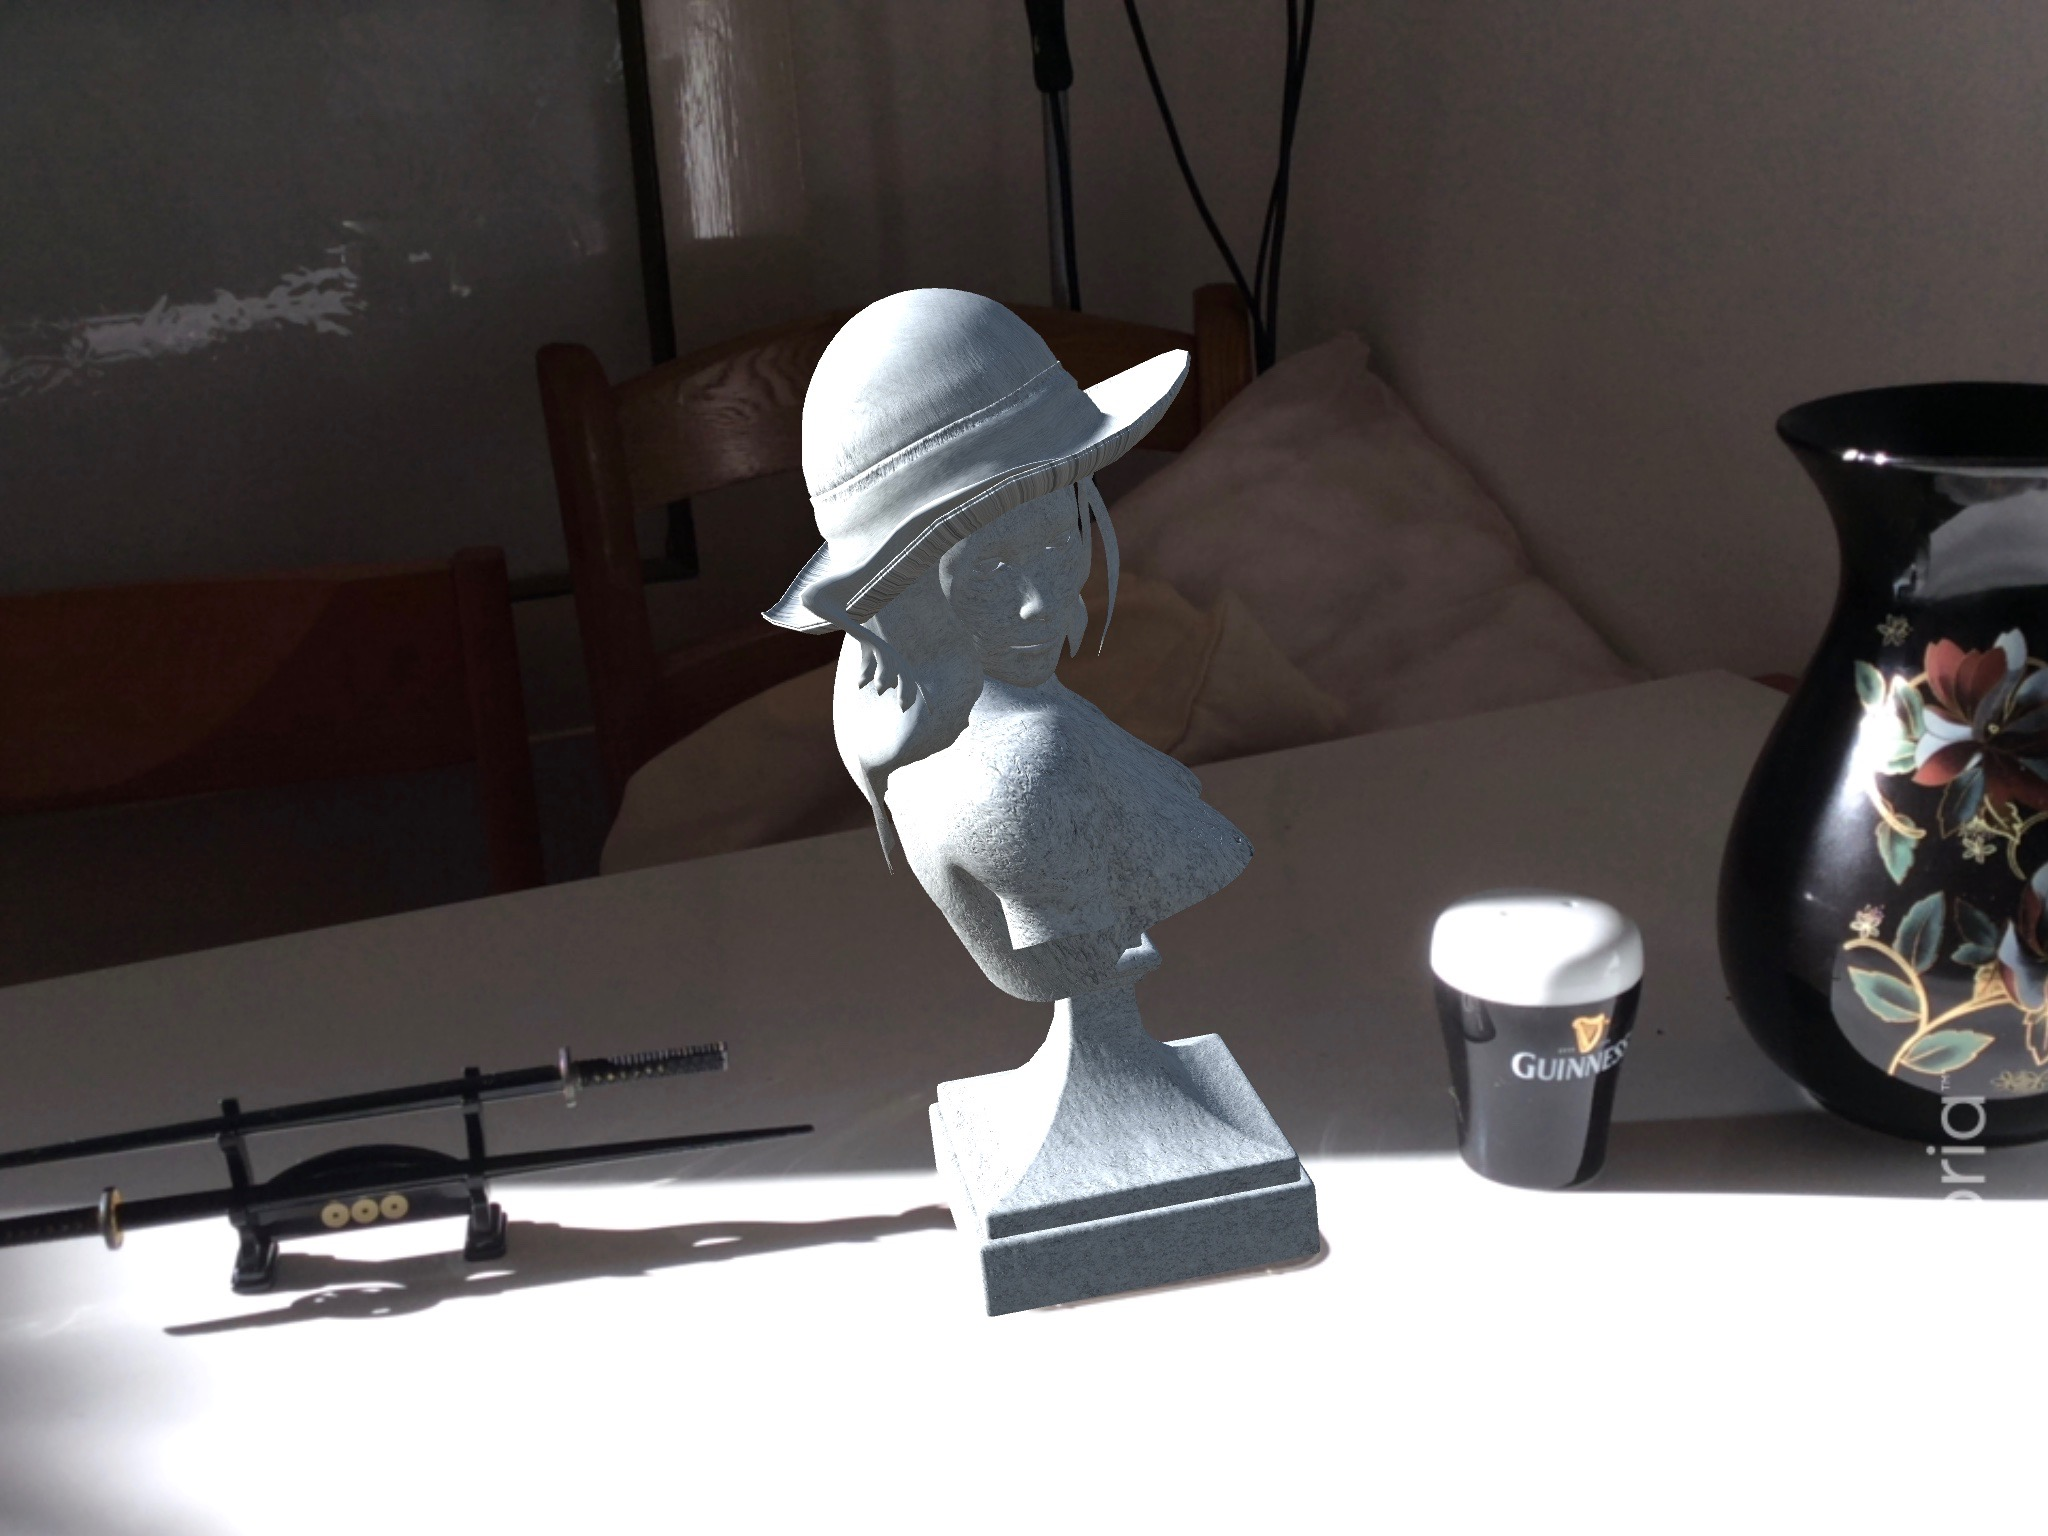
\includegraphics[width=0.6\textwidth]{Figures/realish.jpg}
\caption{Adjusted lighting, giving a more believable look}
\end{figure}
